\documentclass[11pt,a4paper]{article}

\usepackage[a4paper,margin=1in]{geometry}
\usepackage{graphicx}
\usepackage{float}
\usepackage{tabularx}
\usepackage{array}
\usepackage{booktabs}
\usepackage{hyperref}
\usepackage{xcolor}
\usepackage{fancyhdr}
\usepackage{titlesec}
\usepackage{fontspec}
\usepackage{enumitem}
\usepackage{parskip}
\usepackage{caption}
\usepackage{setspace}

\IfFontExistsTF{Georgia}
    {\setmainfont{Georgia}}
    {\IfFontExistsTF{Times New Roman}{\setmainfont{Times New Roman}}{}}

\IfFontExistsTF{Segoe UI}
    {\setsansfont{Segoe UI}}
    {\IfFontExistsTF{Arial}{\setsansfont{Arial}}{}}

\definecolor{DSBlue}{HTML}{173B5D}
\definecolor{DSGold}{HTML}{D79B2E}
\definecolor{DSGreen}{HTML}{2F6B3A}
\definecolor{DSStone}{HTML}{ECE7DC}
\definecolor{DSInk}{HTML}{1A1A1A}

\hypersetup{
    colorlinks=true,
    linkcolor=DSBlue,
    urlcolor=DSBlue,
    pdftitle={Dungeon Surge Spielhandbuch},
    pdfauthor={GitHub Copilot},
    pdfsubject={Illustriertes Spielerhandbuch}
}

\pagestyle{fancy}
\fancyhf{}
\fancyhead[L]{\sffamily\color{DSBlue}Dungeon Surge Handbuch}
\fancyhead[R]{\sffamily\color{DSGold}Illustrierte Ausgabe}
\fancyfoot[C]{\thepage}
\setlength{\headheight}{14pt}

\titleformat{\section}
  {\Large\bfseries\sffamily\color{DSBlue}}
  {\thesection}
  {0.75em}
  {}

\titleformat{\subsection}
  {\large\bfseries\sffamily\color{DSGreen}}
  {\thesubsection}
  {0.75em}
  {}

\captionsetup{
    labelfont={bf,sf,color=DSBlue},
    textfont={small,it}
}

\setlist[itemize]{leftmargin=1.4em}
\setlist[enumerate]{leftmargin=1.6em}
\setstretch{1.05}

\newcommand{\callout}[2]{%
    \noindent\fcolorbox{DSBlue}{DSStone}{%
        \begin{minipage}{0.96\linewidth}
            {\sffamily\bfseries\color{DSBlue}#1}\par
            \vspace{0.2em}
            #2
        \end{minipage}}
}

\newcommand{\manualimage}[3]{%
    \begin{figure}[H]
        \centering
        \fcolorbox{DSBlue}{white}{\includegraphics[width=#2\linewidth]{#1}}
        \caption{#3}
    \end{figure}
}

\begin{document}

\begin{titlepage}
    \centering
    \vspace*{0.8cm}

    {\Huge\bfseries\sffamily\color{DSBlue}Dungeon Surge\par}
    \vspace{0.25cm}
    {\LARGE\sffamily\color{DSGold}Kompaktes Spielhandbuch\par}
    \vspace{0.35cm}
    {\large\color{DSInk}Kämpfen \textbar\ Gold sammeln \textbar\ Aufleveln\par}

    \vspace{0.8cm}
    \fcolorbox{DSBlue}{white}{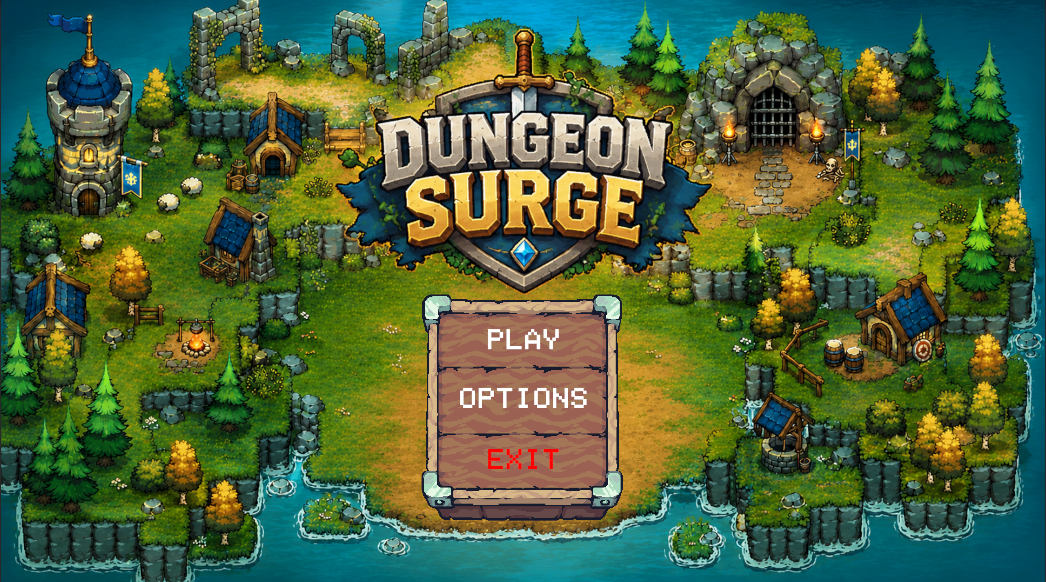
\includegraphics[width=0.96\textwidth]{MainMenu.png}}

    \vfill

    \callout{Kurz gesagt}{
        Zwei Level, zwei Bosse, viele Gegner.\newline
        Sammle Gold, nimm Upgrades und bleib am Leben.
    }

    \vfill
    {\small Wenig Text, klare Bilder, direkt für Spieler.\par}
\end{titlepage}

\section{Schnellstart}

\callout{Ziel}{
Besiege den Goblin-König in Level 1 und die Vampirfledermaus in Level 2.
}

\begin{enumerate}
    \item Starte im Hauptmenü ein neues Spiel.
    \item Besiege Gegner und sammle ihr Gold ein.
    \item Wähle beim Level-Up genau eine Karte.
    \item Besiege nach fünf Wellen den Boss.
\end{enumerate}

\callout{Merksatz}{Gold ist Erfahrung. Viel einsammeln heißt schneller stärker werden.}

\section{Steuerung}

\begin{tabularx}{\linewidth}{@{}>{\bfseries}l X@{}}
    \toprule
    Aktion & Bedienung \\
    \midrule
    Bewegung & Meistens WASD oder Pfeiltasten. \\
    Angriff & Meistens linke Maustaste oder Fire1. \\
    Pause & Escape öffnet das Pausenmenü. \\
    \bottomrule
\end{tabularx}

\vspace{0.8cm}

\begin{figure}[H]
    \centering
    \begin{minipage}[t]{0.47\linewidth}
        \centering
        \fcolorbox{DSBlue}{white}{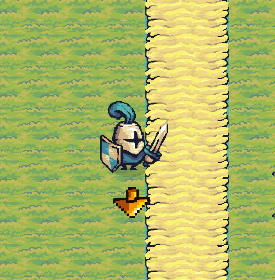
\includegraphics[width=0.92\linewidth]{MainCharackter.png}}
        \caption{Der Held in Bewegung.}
    \end{minipage}\hfill
    \begin{minipage}[t]{0.47\linewidth}
        \centering
        \fcolorbox{DSBlue}{white}{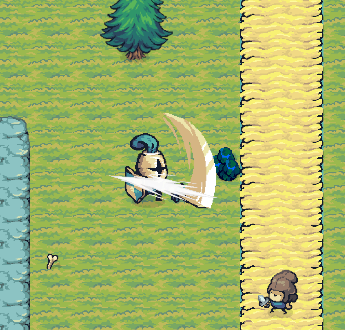
\includegraphics[width=0.92\linewidth]{MainCharakter_Attack.png}}
        \caption{Nahkampfangriff im Einsatz.}
    \end{minipage}
\end{figure}

\section{Kampf}

Dein Held kämpft im Nahbereich.

\begin{itemize}
    \item Bleib nah am Ziel.
    \item Treffer haben Timing.
    \item Feindtreffer können dich zurückstoßen.
    \item Bei Bossauftritten bist du kurzzeitig ohne Kontrolle.
    \item Bei null Leben ist der Lauf vorbei.
\end{itemize}

\section{Level-Up}

Beim Stufenaufstieg pausiert das Spiel. Wähle eine Karte.

\manualimage{LevelUpMenu.png}{0.90}{Ein Level-Up zeigt mehrere Karten, aber du nimmst nur eine.}

\begin{figure}[H]
    \centering
    \begin{minipage}[t]{0.31\linewidth}
        \centering
        \fcolorbox{DSBlue}{white}{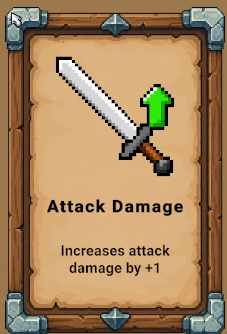
\includegraphics[width=0.95\linewidth]{AttackMenu.png}}
        \caption{Angriff}
    \end{minipage}\hfill
    \begin{minipage}[t]{0.31\linewidth}
        \centering
        \fcolorbox{DSBlue}{white}{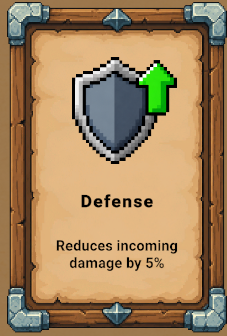
\includegraphics[width=0.95\linewidth]{DefenseLevelup.png}}
        \caption{Verteidigung}
    \end{minipage}\hfill
    \begin{minipage}[t]{0.31\linewidth}
        \centering
        \fcolorbox{DSBlue}{white}{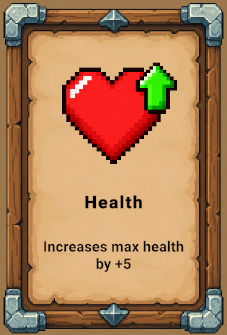
\includegraphics[width=0.95\linewidth]{HealthLevelup.png}}
        \caption{Leben}
    \end{minipage}
\end{figure}

\callout{Weitere Boni}{Tempo und Regeneration können ebenfalls auftauchen.}

\section{Leben und Schutz}

\begin{itemize}
    \item Verteidigung senkt den eingehenden Schaden.
    \item Max. Leben vergrößert deinen Vorrat.
    \item Regeneration heilt mit der Zeit.
    \item Verteidigung wächst nicht endlos.
\end{itemize}

\section{Level und Bosse}

Dein Lauf hat zwei Level.

\begin{tabularx}{\linewidth}{@{}>{\bfseries}l c l X@{}}
    \toprule
    Abschnitt & Wellen & Boss & Danach \\
    \midrule
    Level 1 & 5 & Goblin-König & Der Abschnitt endet und dein Fortschritt geht mit nach Level 2. \\
    Level 2 & 5 & Vampirfledermaus & Nach dem Sieg endet der Lauf und du kehrst ins Hauptmenü zurück. \\
    \bottomrule
\end{tabularx}

\begin{figure}[H]
    \centering
    \begin{minipage}[t]{0.47\linewidth}
        \centering
        \fcolorbox{DSBlue}{white}{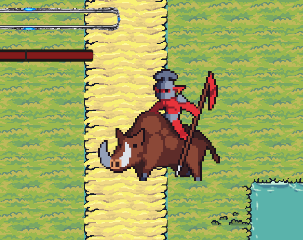
\includegraphics[width=0.92\linewidth]{BOss1.png}}
        \caption{Der Goblin-König in Level 1.}
    \end{minipage}\hfill
    \begin{minipage}[t]{0.47\linewidth}
        \centering
        \fcolorbox{DSBlue}{white}{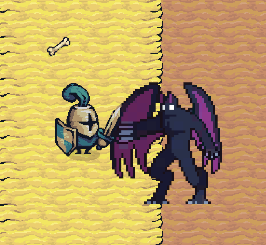
\includegraphics[width=0.92\linewidth]{boss2.png}}
        \caption{Die Vampirfledermaus in Level 2.}
    \end{minipage}
\end{figure}

\callout{Bossregel}{Erst alle Wellen, dann der Boss.}

\section{Menüs und Bildschirme}

\begin{figure}[H]
    \centering
    \begin{minipage}[t]{0.58\linewidth}
        \centering
        \fcolorbox{DSBlue}{white}{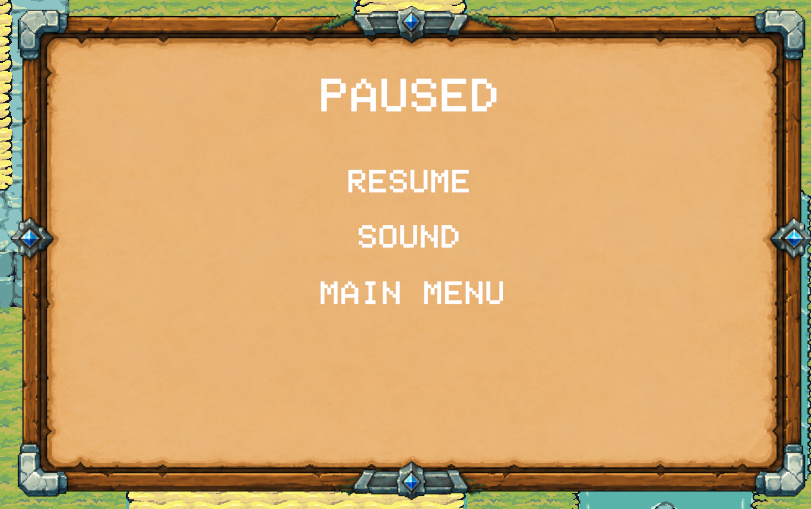
\includegraphics[width=0.95\linewidth]{PauseMenu.png}}
        \caption{Pausenmenü}
    \end{minipage}\hfill
    \begin{minipage}[t]{0.34\linewidth}
        \centering
        \fcolorbox{DSBlue}{white}{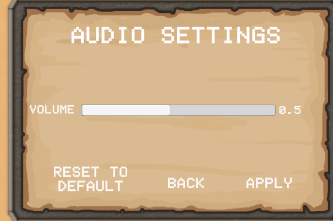
\includegraphics[width=0.95\linewidth]{SoundSettings.png}}
        \caption{Sound-Einstellungen}
    \end{minipage}
\end{figure}

\begin{itemize}
    \item Hauptmenü: Neues Spiel, Optionen, Beenden.
    \item Pause: Fortsetzen, Sound, Hauptmenü.
    \item Sound: Lautstärke ändern, anwenden oder zurücksetzen.
\end{itemize}

\section{Kurz-Tipps}

\begin{itemize}
    \item Lass kein Gold liegen.
    \item Erst Überleben, dann Schaden.
    \item Mehr Tempo hilft gegen volle Wellen.
    \item Spiel ruhig, nicht hektisch.
\end{itemize}

\end{document}